%% (Master) Thesis template
% Template version used: v1.4
%
% Largely adapted from Adrian Nievergelt's template for the ADPS
% (lecture notes) project.


%% We use the memoir class because it offers a many easy to use features.
\documentclass[11pt,a4paper,titlepage]{memoir}

%% Packages
%% ========

%% LaTeX Font encoding -- DO NOT CHANGE
\usepackage[OT1]{fontenc}

%% Babel provides support for languages.  'english' uses British
%% English hyphenation and text snippets like "Figure" and
%% "Theorem". Use the option 'ngerman' if your document is in German.
%% Use 'american' for American English.  Note that if you change this,
%% the next LaTeX run may show spurious errors.  Simply run it again.
%% If they persist, remove the .aux file and try again.
\usepackage[english]{babel}

%% Input encoding 'utf8'. In some cases you might need 'utf8x' for
%% extra symbols. Not all editors, especially on Windows, are UTF-8
%% capable, so you may want to use 'latin1' instead.
\usepackage[utf8]{inputenc}

%% This changes default fonts for both text and math mode to use Herman Zapfs
%% excellent Palatino font.  Do not change this.
\usepackage[sc]{mathpazo}

%% The AMS-LaTeX extensions for mathematical typesetting.  Do not
%% remove.
\usepackage{amsmath,amssymb,amsfonts,mathrsfs}

%% NTheorem is a reimplementation of the AMS Theorem package. This
%% will allow us to typeset theorems like examples, proofs and
%% similar.  Do not remove.
%% NOTE: Must be loaded AFTER amsmath, or the \qed placement will
%% break
\usepackage[amsmath,thmmarks]{ntheorem}

%% LaTeX' own graphics handling
\usepackage{graphicx}

%% Better arrange figures.
\usepackage{float}

%% Be able to draw svg's.
\usepackage{svg}

%% We unfortunately need this for the Rules chapter.  Remove it
%% afterwards; or at least NEVER use its underlining features.
\usepackage{soul}

%% This allows you to add .pdf files. It is used to add the
%% declaration of originality.
\usepackage{pdfpages}

%% Some more packages that you may want to use.  Have a look at the
%% file, and consult the package docs for each.
%% See the TeXed file for more explanations

%% [OPT] Multi-rowed cells in tabulars
%\usepackage{multirow}

%% [REC] Intelligent cross reference package. This allows for nice
%% combined references that include the reference and a hint to where
%% to look for it.
\usepackage{varioref}

%% [OPT] Easily changeable quotes with \enquote{Text}
%\usepackage[german=swiss]{csquotes}

%% [REC] Format dates and time depending on locale
\usepackage{datetime}

%% [OPT] Provides a \cancel{} command to stroke through mathematics.
%\usepackage{cancel}

%% [NEED] This allows for additional typesetting tools in mathmode.
%% See its excellent documentation.
\usepackage{mathtools}

%% [ADV] Conditional commands
%\usepackage{ifthen}

%% [OPT] Manual large braces or other delimiters.
%\usepackage{bigdelim, bigstrut}

%% [REC] Alternate vector arrows. Use the command \vv{} to get scaled
%% vector arrows.
\usepackage[h]{esvect}

%% [NEED] Some extensions to tabulars and array environments.
\usepackage{array}

%% [OPT] Postscript support via pstricks graphics package. Very
%% diverse applications.
%\usepackage{pstricks,pst-all}

%% [?] This seems to allow us to define some additional counters.
%\usepackage{etex}

%% [ADV] XY-Pic to typeset some matrix-style graphics
%\usepackage[all]{xy}

%% [OPT] This is needed to generate an index at the end of the
%% document.
%\usepackage{makeidx}

%% [OPT] Fancy package for source code listings.  The template text
%% needs it for some LaTeX snippets; remove/adapt the \lstset when you
%% remove the template content.
\usepackage{listings}
\lstset{language=TeX,basicstyle={\normalfont\ttfamily}}

%% [REC] Fancy character protrusion.  Must be loaded after all fonts.
\usepackage[activate]{pdfcprot}

%% [REC] Nicer tables.  Read the excellent documentation.
\usepackage{booktabs}


%% Our layout configuration.  DO NOT CHANGE.
%% Memoir layout setup

%% NOTE: You are strongly advised not to change any of them unless you
%% know what you are doing.  These settings strongly interact in the
%% final look of the document.

% Dependencies
\usepackage{ETHlogo}

% Turn extra space before chapter headings off.
\setlength{\beforechapskip}{0pt}

\nonzeroparskip
\parindent=0pt
\defaultlists

% Chapter style redefinition
\makeatletter

\if@twoside
  \pagestyle{Ruled}
  \copypagestyle{chapter}{Ruled}
\else
  \pagestyle{ruled}
  \copypagestyle{chapter}{ruled}
\fi
\makeoddhead{chapter}{}{}{}
\makeevenhead{chapter}{}{}{}
\makeheadrule{chapter}{\textwidth}{0pt}
\copypagestyle{abstract}{empty}

\makechapterstyle{bianchimod}{%
  \chapterstyle{default}
  \renewcommand*{\chapnamefont}{\normalfont\Large\sffamily}
  \renewcommand*{\chapnumfont}{\normalfont\Large\sffamily}
  \renewcommand*{\printchaptername}{%
    \chapnamefont\centering\@chapapp}
  \renewcommand*{\printchapternum}{\chapnumfont {\thechapter}}
  \renewcommand*{\chaptitlefont}{\normalfont\huge\sffamily}
  \renewcommand*{\printchaptertitle}[1]{%
    \hrule\vskip\onelineskip \centering \chaptitlefont\textbf{\vphantom{gyM}##1}\par}
  \renewcommand*{\afterchaptertitle}{\vskip\onelineskip \hrule\vskip
    \afterchapskip}
  \renewcommand*{\printchapternonum}{%
    \vphantom{\chapnumfont {9}}\afterchapternum}}

% Use the newly defined style
\chapterstyle{bianchimod}

\setsecheadstyle{\Large\bfseries\sffamily}
\setsubsecheadstyle{\large\bfseries\sffamily}
\setsubsubsecheadstyle{\bfseries\sffamily}
\setparaheadstyle{\normalsize\bfseries\sffamily}
\setsubparaheadstyle{\normalsize\itshape\sffamily}
\setsubparaindent{0pt}

% Set captions to a more separated style for clearness
\captionnamefont{\sffamily\bfseries\footnotesize}
\captiontitlefont{\sffamily\footnotesize}
\setlength{\intextsep}{16pt}
\setlength{\belowcaptionskip}{1pt}

% Set section and TOC numbering depth to subsection
\setsecnumdepth{subsection}
\settocdepth{subsection}

%% Titlepage adjustments
\pretitle{\vspace{0pt plus 0.7fill}\begin{center}\HUGE\sffamily\bfseries}
\posttitle{\end{center}\par}
\preauthor{\par\begin{center}\let\and\\\Large\sffamily}
\postauthor{\end{center}}
\predate{\par\begin{center}\Large\sffamily}
\postdate{\end{center}}

\def\@advisors{}
\newcommand{\advisors}[1]{\def\@advisors{#1}}
\def\@department{}
\newcommand{\department}[1]{\def\@department{#1}}
\def\@thesistype{}
\newcommand{\thesistype}[1]{\def\@thesistype{#1}}

\renewcommand{\maketitlehooka}{\noindent\ETHlogo[2in]}

\renewcommand{\maketitlehookb}{\vspace{1in}%
  \par\begin{center}\Large\sffamily\@thesistype\end{center}}

\renewcommand{\maketitlehookd}{%
  \vfill\par
  \begin{flushright}
    \sffamily
    \@advisors\par
    \@department, ETH Z\"urich
  \end{flushright}
}

\checkandfixthelayout

\setlength{\droptitle}{-48pt}

\makeatother

% This defines how theorems should look. Best leave as is.
\theoremstyle{plain}
\setlength\theorempostskipamount{0pt}

%%% Local Variables:
%%% mode: latex
%%% TeX-master: "thesis"
%%% End:


%% Theorem environments.  You will have to adapt this for a German
%% thesis.
%% Theorem-like environments

%% This can be changed according to language. You can comment out the ones you
%% don't need.

\numberwithin{equation}{chapter}

%% German theorems
%\newtheorem{satz}{Satz}[chapter]
%\newtheorem{beispiel}[satz]{Beispiel}
%\newtheorem{bemerkung}[satz]{Bemerkung}
%\newtheorem{korrolar}[satz]{Korrolar}
%\newtheorem{definition}[satz]{Definition}
%\newtheorem{lemma}[satz]{Lemma}
%\newtheorem{proposition}[satz]{Proposition}

%% English variants
\newtheorem{theorem}{Theorem}[chapter]
\newtheorem{example}[theorem]{Example}
\newtheorem{remark}[theorem]{Remark}
\newtheorem{corollary}[theorem]{Corollary}
\newtheorem{definition}[theorem]{Definition}
\newtheorem{lemma}[theorem]{Lemma}
\newtheorem{proposition}[theorem]{Proposition}

%% Proof environment with a small square as a "qed" symbol
\theoremstyle{nonumberplain}
\theorembodyfont{\normalfont}
\theoremsymbol{\ensuremath{\square}}
\newtheorem{proof}{Proof}
%\newtheorem{beweis}{Beweis}


%% Helpful macros.
%% Custom commands
%% ===============

%% Special characters for number sets, e.g. real or complex numbers.
\newcommand{\C}{\mathbb{C}}
\newcommand{\K}{\mathbb{K}}
\newcommand{\N}{\mathbb{N}}
\newcommand{\Q}{\mathbb{Q}}
\newcommand{\R}{\mathbb{R}}
\newcommand{\Z}{\mathbb{Z}}
\newcommand{\X}{\mathbb{X}}

%% Fixed/scaling delimiter examples (see mathtools documentation)
\DeclarePairedDelimiter\abs{\lvert}{\rvert}
\DeclarePairedDelimiter\norm{\lVert}{\rVert}

%% Use the alternative epsilon per default and define the old one as \oldepsilon
\let\oldepsilon\epsilon
\renewcommand{\epsilon}{\ensuremath\varepsilon}

%% Also set the alternate phi as default.
\let\oldphi\phi
\renewcommand{\phi}{\ensuremath{\varphi}}


\graphicspath{ {./images/} }


%% Make document internal hyperlinks wherever possible. (TOC, references)
%% This MUST be loaded after varioref, which is loaded in 'extrapackages'
%% above.  We just load it last to be safe.
\usepackage[linkcolor=black,colorlinks=true,citecolor=black,filecolor=black]{hyperref}


%% Document information
%% ====================

\title{Multi-model disentanglement of object representation}
\author{Eric Stavarache}
\thesistype{Master Thesis}
\advisors{Advisors: Frederik Benzing, Asier Mujika}
\department{Department of Computer Science}
\date{July 19, 2019}

\begin{document}

\frontmatter

%% Title page is autogenerated from document information above.  DO
%% NOT CHANGE.
\begin{titlingpage}
  \calccentering{\unitlength}
  \begin{adjustwidth*}{\unitlength-24pt}{-\unitlength-24pt}
    \maketitle
  \end{adjustwidth*}
\end{titlingpage}

%% The abstract of your thesis.  Edit the file as needed.
\begin{abstract}
  This example thesis briefly shows the main features of our thesis
  style, and how to use it for your purposes.
\end{abstract}


%% TOC with the proper setup, do not change.
\cleartorecto
\tableofcontents
\mainmatter

\chapter{Introduction}

Humans reason about the surrounding world by decomposing it into orthogonal components.
The idea of an object is decoupled from the qualities of the object: it is very
easy for us to imagine a pink elephant, even though we have never observed such
an animal, and these two words suffice for us to imagine a visual scene.
The words are a latent representation of the scene.

Variational Autoencoders (VAE) \cite{bib:vae_paper} are a powerful framework for
learning latent representations. Much work has already been done on disentangled
representations, where we require that any two latent variables are uncorrelated.

Our work focuses on model-based disentanglement of objects. In particular, we
would like to have one individual VAE which is trained to recognise and
represent a single type of object: in a normal setting, we could have one VAE
which represents chairs, another VAE which represents tables, and so on.
We will call our approach the \textbf{SuperVAE}.

Most similar in spirit is the \cite{bib:monet}, where a single VAE model
iteratively recognises objects from a scene by using attention masks.
The main difference is that the MONet uses a single VAE for all objects, whereas
we use multiple VAE's in parallel.
Another similar idea is contained in \cite{bib:iodine}, where they have a single
VAE which tries to model the scene, and where they iteratively refine the latent
parameters.

\chapter{Method}

\section{SuperVAE}


The SuperVAE network tries to reconstructor a scene by feeding the image to some
VAE's connected in parallel, whereby every VAE models a separate part of the scene.


Let us say that there are $K$ VAE's, where each of them tries to model a
different object.
Then the image $X$ will be fed independently to
each of them.

Each VAE will then model a distribution over the latent variables,
$q_{\theta_k}(\textbf{z}_k | \textbf{X})$.

By sampling from these distribution, they will generate two outputs of
the same size as the image: $\hat{X}_k$, which is the $k$'th model
reconstruction of the image, and $\hat{m}_{k}$, which is a confidence mask.

This confidence mask represents how sure a VAE is about its output for a given
pixel. Higher confidence means that the pixel is part of an object which is of
the type the VAE is modelling.

These confidence masks are produced by first having the models generate some
``raw'' confidence values, and then taking a pixel-wise softmax across all of
the $k$ models.

Thus, the masks are a probability distribution, where for each pixel we have
what is the probability that it belongs to an object modelled by a VAE:

$\sum_{i = 1}^{k} \hat{m}_{k} = \textbf{1}$.

\begin{figure}
  \caption{A diagram of how the model operates.}
  \includegraphics[scale=0.7]{model.png}
\end{figure}

Our loss function is

\[
  \mathcal{L}(X; \theta _1, ..., \theta_k) =
  \sum_{i = 1}^{k}
  \norm {
    (\hat{X}_{i} - X)
    \odot \hat{m}_{i}
  }^2_F
  +
  \beta \sum_{i = 1}^{k} D_{KL} [ q_{\theta_k} (\textbf{z}_k | \textbf{X}) ||
  \mathcal{N}(0, \mathbf{I}) ]
  +
  \gamma \cdot - \log (
  \frac{1} {\log{K}}
  \cdot - \hat{m} \log {\hat{m}}
  )
\]

The first term of the loss is a $L_2$ loss weighted by each model's confidence.
The intuition behind this is that the more responsability a VAE takes for
drawing certain pixel, the more it should be penalized for making mistakes.

The second term is the standard KL loss term, weighted by a $\beta$
hyperparameter, as first introduced in \cite{bib:betavae}.

The last term is our original contribution, which is a cross-entropy loss.
The idea is that the VAE's should try to be unassuming, and they should incur a
cost if they decide to take on a lot of responsability for representing a pixel.
We have the $-\hat{m} \log {\hat{m}}$ term, which is the normal cross-entropy,
where we interpret the masks as component-wise distributions over VAE's.
We divide it by the maximal value it can take ($\log{K}$, where $K$ is the
number of VAE's) in order to obtain a value between $0$ and $1$.
We want to penalize situations where one VAE takes over everything, and in these
situations the cross-entropy would be close to $0$. As such, we take the
negative log of the normalized cross-entropy.
This whole term is weighted by another hyperparameter, $\gamma$.


We compare this with the approach of \cite{bib:monet}, where they have a single
VAE which tries to model all objects, whereas we have a single VAE for each
object type.
Furthermore, in their model, the VAE is instructed what to model by the U-Net
attention mask, whereas in our approach each VAE decides ``independently'' what
to learn. In our approach, the only communication happening between the VAE's is
via the softmax operation of the confidence masks.


\chapter{Results}

For our experiments, we have taken a supervised approach to training the models.

\section{MNIST}

In order to test our idea, we began with the MNIST dataset.
To make the task more challenging, and to allow decomposition via objects, we
construct our training data by putting two digits side-by-side.

\subsection{2-MNIST}

At the start, we set up only 2 VAE's in parallel, where we want that VAE-0 learns to
recognise and model the digit 0, and VAE-1 models digit 1.

In order to accomplish this, we split the training into two stages:

\begin{enumerate}
  \item In stage 0, VAE-0 trains on reconstructing images containing
    only the digit $0$. The other model is active (so they are contributing
    to the confidence masks), but its weights are frozen, and only
    VAE-0 is learning.
  \item In stage 1, VAE-1 trains on images containing digits $0$ and $1$ (so of
    the two slots, each digit is sampled independently). In this time, VAE-0 is
    frozen, \textit{however} it is still contributing to the confidence masks.
    Because of this, places where the digit $0$ appears are already assigned
    high confidence values by VAE-0, and so VAE-1 will not be motivated to learn
    them. On the other hand, places where digit 1 appears will not be recognised
    by VAE-0, and so VAE-1 will learn them.
\end{enumerate}

\begin{figure}[H]
  \label{fig:2mnist}
  \caption{Results of training on 2-MNIST.
    Each picture has 6 rows: first row is input image $X$, second row is
    confidence mask of VAE-0 $\hat{m}_{0}$, third row is reconstruction of VAE-0
    $\hat{X}_{0}$, fourth row is $\hat{m}_{1}$, fifth row is $\hat{X}_{1}$, and
    last row is weighted reconstruction.
  }
  \centering
  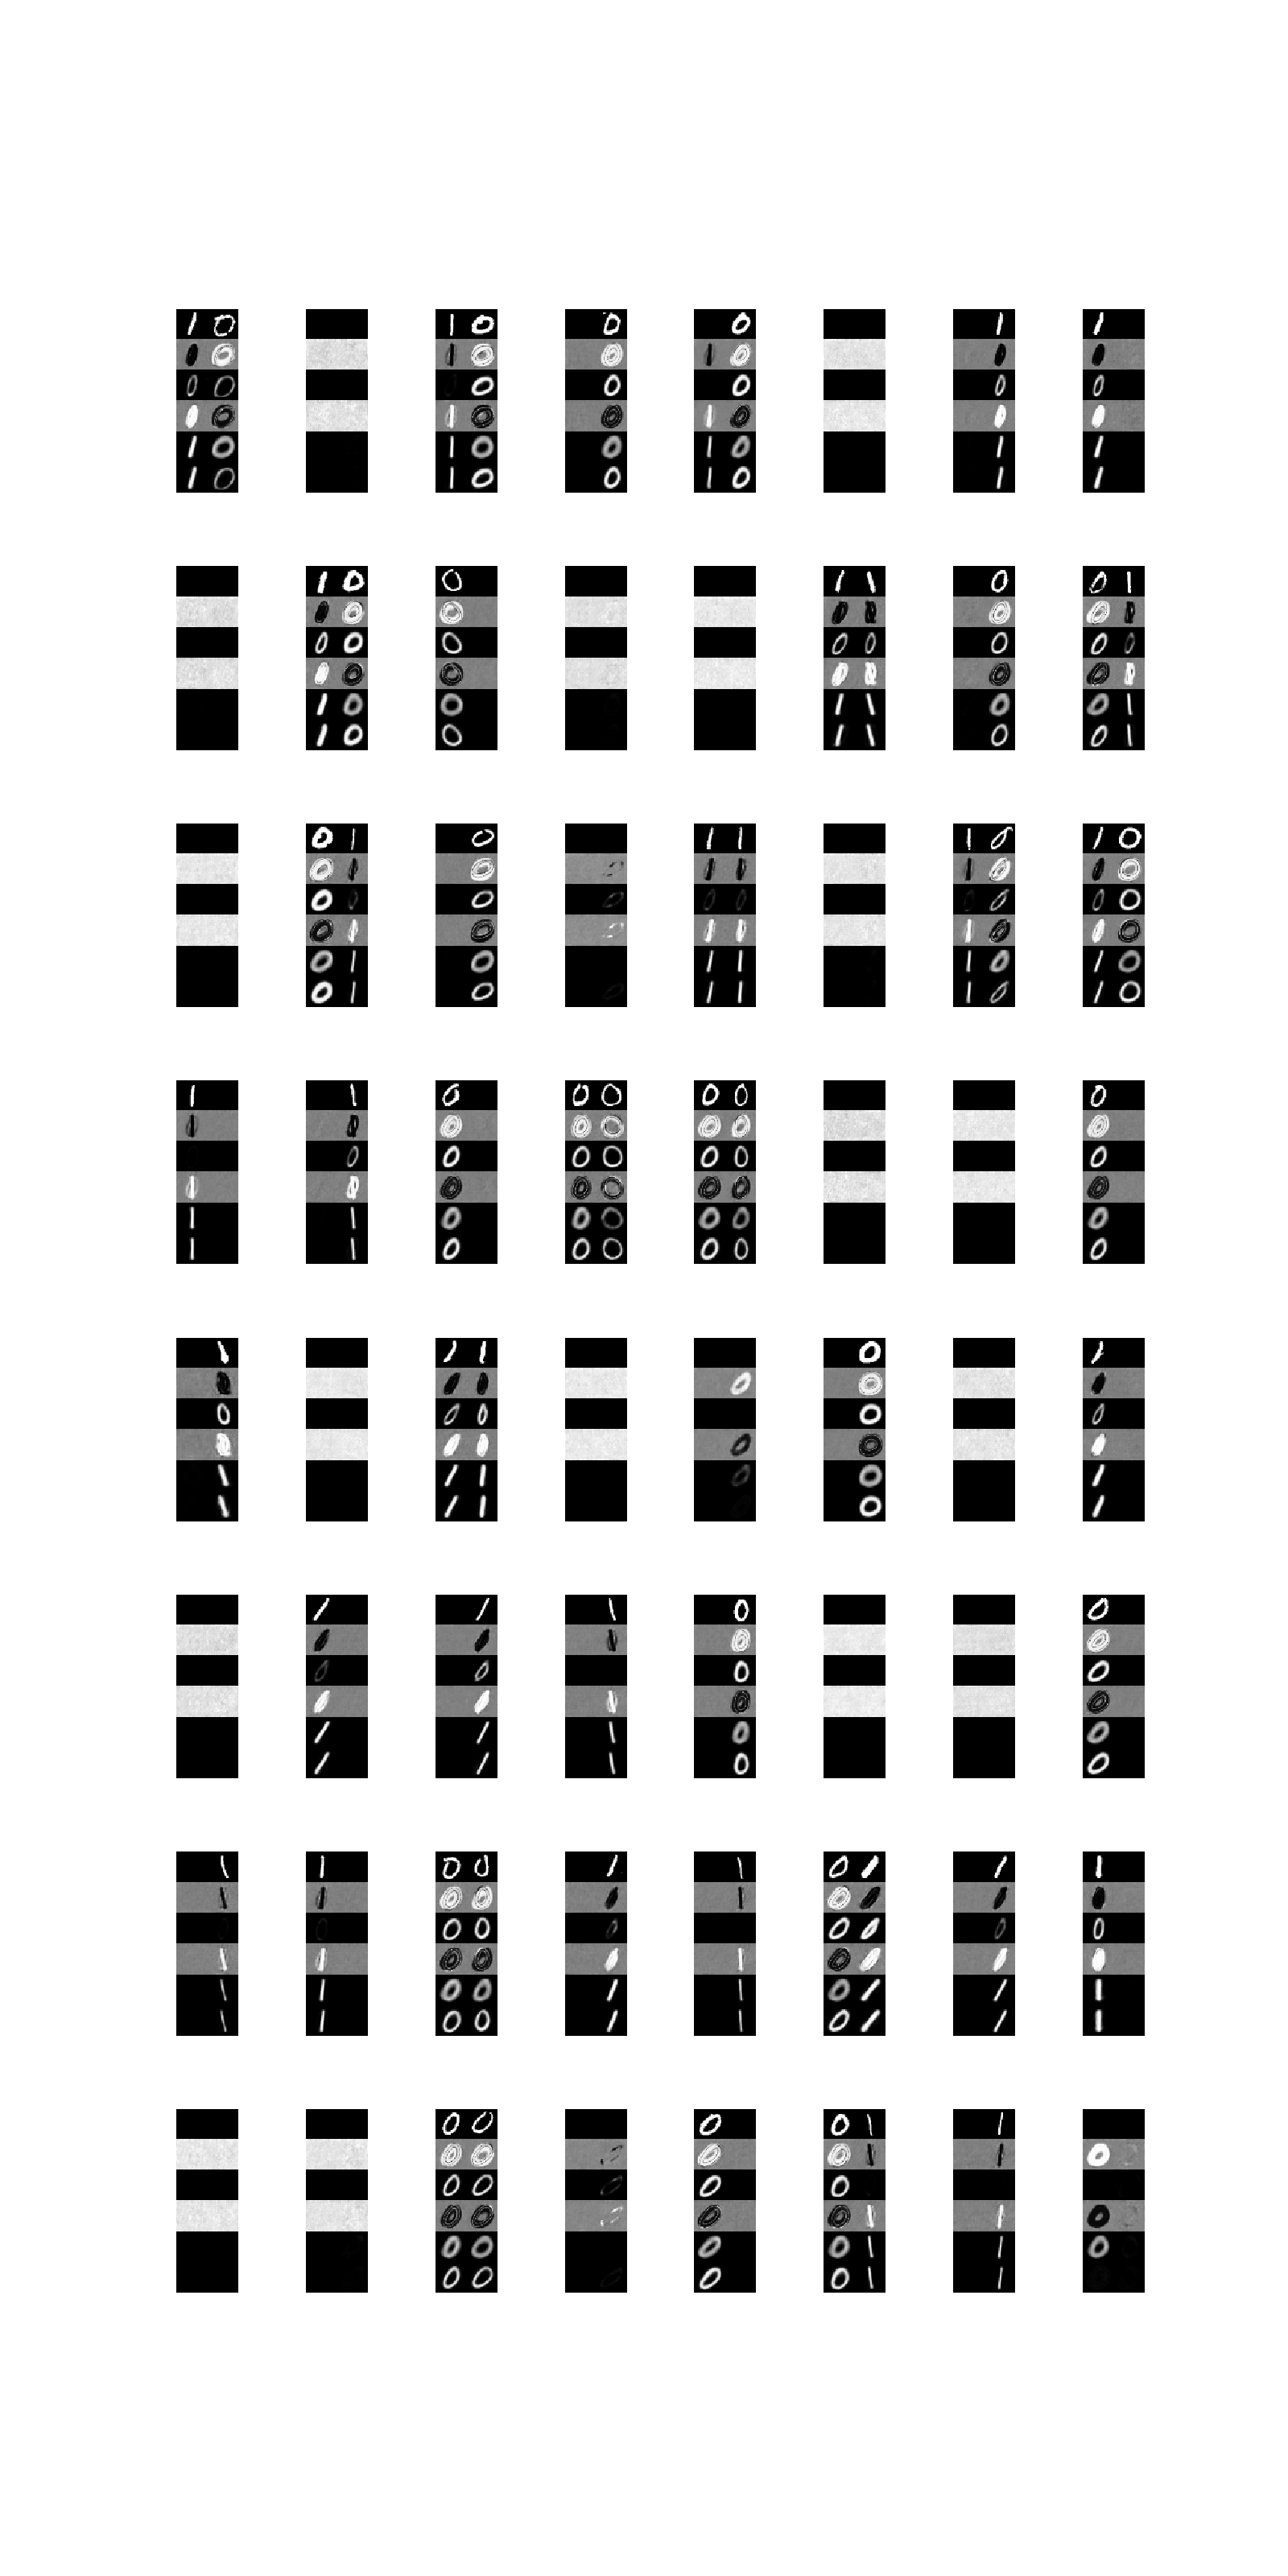
\includegraphics[scale=0.3]{init_progress.png}
\end{figure}

As we can see in figure \ref{fig:2mnist}, we have the desired effect: VAE 0 has
high confidences (indicated by very white portions of the confidence mask) where
the digit 0 appears, and has VAE 1 has high confidences where the digit 1 appears.

We note that there are cases when, even though VAE 0 has low confidence, it
still draws a 0. This is because it was trained only on zeroes, so when
encountering a digit 1 it does the only thing it knows how to do: output a 0.
Similarly, VAE 1 draws very generic zeroes when the input digit is a 0. Since it
was trained on both images of 0 and 1, it has had a chance to learn how a
generic 0 looks like. Furthermore, it only takes one bit of information to store
if the input is a $0$ (which is then included in the KL-loss), but it has a lot
to gain by making its reproduction closer to the original image (which is the
first term in the overall loss function).

After this experiment, we then proceeded to see what would happen with $5$ VAE's
in parallel.

\subsection{5-MNIST}

For this dataset, we again have the same two digit side-by-side training data.
However, we now have $5$ VAE's wired up together, where again we would want that
VAE $i$ learns to model digit $i$.

The training is done analogous to 2-MNIST, in $5$ stages, where in stage $k$
model $k$ is learning by looking at images containing digits $0, 1, ..., k$, and
all of the other models are frozen (but still contributing to the confidences).

\begin{figure}[H]
  \label{fig:5mnist}
  \caption{Results of training on 5-MNIST.
    Each picture has 12 rows: first row is input image $X$, last row is
    reconstructed image.
    In between, each adjacent pair of rows represents the confidences
    $\hat{m}_k$ and the reconstructions $\hat{X}_k$ for each of the $K = 5$ VAE's.
    Note that even though the digit $5$ appears as part of the input, none of
    the models were trained on it: this is just test data. We include it only to
    see how models generalize to unseen digits.
  }
  \centering
  \includegraphics[scale=0.3]{5-mnist.png}
\end{figure}

From figure \ref{fig:5mnist}, we can see that the model achieves good
reconstructions on the digits which it was trained on.

Again, we observe that when a digit $4$ appears, only the last model has high
confidences, and produces a good reconstruction; the other models generate a
digit which they have learned, which minimizes the $L_2$ loss.

For digit $5$, we observe that the model with the closest digit (in $L_2$ norm)
has high confidence: sometimes the model for $2$, and sometimes the model for
$3$.

\subsection{Alternative training}

\appendix

\chapter{Dummy Appendix}


\backmatter

\bibliographystyle{plain}
\bibliography{refs}

% 
\includepdf[pages={-}]{declaration-originality.pdf}

\end{document}
